\documentclass[table,color,cover,twoside,nolot,nolof]{fithesis3/fithesis3}
\usepackage[english]{babel}
\usepackage{amsmath}
\usepackage{tabularx}
\usepackage{booktabs}
\usepackage{graphics}
\usepackage{caption}
\usepackage{subcaption}
\usepackage{numprint}
\usepackage{bibentry}
\usepackage[inline]{enumitem}
\nobibliography*
\thesissetup{
	faculty=fi,
	title=Computerized Adaptive Practice of Factual Knowledge,
	type=p,
	author=Jan Papou\v{s}ek,
	advisor=Radek Pel\'{a}nek,
	keywords={varied prior knowledge, adaptive educational system, intelligent
		tutoring system, computerized adaptive practice, factual knowledge, task
		construction},
	basePath=./fithesis3
}
\usepackage[final]{pdfpages}
\usepackage{tabularx}
\usepackage[inline]{enumitem}

\makeatletter\thesis@load\makeatother
\setcounter{tocdepth}{2}

\begin{document}

\chapter{Introduction}

Using computers and other electronic devices becomes more and mo\-re common in
every day life. It is thus natural to use them also in the~domain of
education. We can look at this kind of their application in two different
viewpoints. In the first case they are used to help teachers to spend less
time doing routine tasks and more time with students, to prepare good teaching
materials, to effectively find out what students know and what they do not
know, and so on. Of course this has indirect positive impact on students. In
the second case computers may help students directly as they can serve as a
platform where personalized systems provide adaptive content, e.g.~guide
students in situations when they lag behind or introduce new challenges when
they are able to solve the previous ones. To understand how these systems are
used it is important to realize students usually interact with them with
minimal assistance of teachers.

Although the first case is important we focus on the second one, i.e. on the
way computers can help students directly. We are mainly interested in systems
where students actively solve presented tasks, i.e. in systems for
\emph{computerized adaptive practice}~\cite{klinkenberg2011computer}. According
to~\cite{vanlehn2006behavior} this kind of practice consists of two loops. The
outer loop describes selection of a task to solve and in case of the inner one
a system guides its users in the process of solution of a complex multi-step
task. As the thesis deals with memorizing facts, e.g. vocabulary or
geographical and anatomical terms, that can be done through atomic tasks
without any intermediate steps, the inner loop is not so important for us. The
considered method of practice consists of answering multiple-choice and open
questions, interleaved with a~feedback on the correctness of answers.

Computerized adaptive practice is one way of self-testing. Based on recent
research~\cite{bjork2013self} self-testing is a~good strategy that may boost
students' performance. On the other side people make a lot of mistakes during
the self-testing. They overestimate their knowledge and this overconfidence
leads to worse choice of tasks for
practice~\cite{bjork2013self,kornell2008optimising}. This makes the practice
less efficient than it could be. The second problematic aspect of self-testing
is that although the repetition is good for memorizing, it is not so commonly
used neither by high performers who may not need it, nor by low performers who
are not motivated to use it~\cite{bjork2013self}. A well-designed system for
computerized adaptive practice can address both of these issues. Moreover this
system can operate online and be available to a large number of users, thus
making self-testing a very natural way to learn.

However, in online educational environments we deal with a lot of different
categories of users. It is natural these systems are used by students,
sometimes even at schools for a fixed amount of time. On the other side they
are also open to non-school users willing to improve their knowledge in their
free time. Having diverse set of users means these users have varied
background, motivation and prior knowledge. Whereas some users may want to
learn for a tomorrow exam, others may be more interested in using their
knowledge in the long term. This contrasts with classical educational
environments, i.e. schools, where learners and their motivation do not differ
so much. For that reason the online system providing the practice has to
attract and keep attention of all kinds of users and ensure they spend
their time in the most efficient way with respect to learning. This can be a
bit difficult, because a strategy motivating users to stay active may be
different from a strategy making the practice efficient with respect to
learning.

To provide adaptivity we need to build an adequate model describing user's
knowledge. The model should take into account e.g. prior knowledge, learning or
forgetting. We also need to design a good strategy for practicing, which may
differ for different types of users. We can not design a~good strategy for
practicing when we are not able to measure its impact on a user's motivation and
its efficiency with respect to learning. It is thus crucial to collect data
about users' activity and evaluate it. This turns out to be a big
methodological issue in online environment.

This issue may or may not have been addressed by commercial systems operating
in this area. Unfortunately the functioning of these systems --
e.g.~\url{www.memrise.com} and \url{www.cerego.com} providing practice of
individual terms within several domains, or
\url{www.duolingo.com}~\cite{garcia2013learning} teaching users foreign
languages by asking them to translate sentences (both in writing and in spoken
word) -- is not often properly described. There are, of course, a few
exceptions, like~\cite{streeter2015mixture}.

The aim of the thesis is to address mentioned issues -- student modeling,
strategies for practice control and evaluation -- to make learning of factual
knowledge more efficient. The outcomes of the thesis will be applied and
evaluated in an online environment, which means they may potentially have a big
impact on learning of a large number of people. They can be also scientifically
influential as they may provide certain hints on the modeling of learning and
on the evaluation methodology.

The state of the art described in Chapter
\ref{chapter:state_of_the_art} is focused on the following three pillars:
\begin{enumerate*}[label=(\arabic*)]
	\item models describing a learner's knowledge and learning;
	\item strategies controlling the practice;
	\item methodologies for evaluation.
\end{enumerate*}
Chapter~\ref{chapter:aims_of_the_thesis} discusses aims of the thesis, its
objectives and the plan of work in more detail.
Chapter~\ref{chapter:achieved_results} consists of brief description of
achieved results.

\chapter{State of the Art}
\label{chapter:state_of_the_art}

Development of a fully adaptive system providing a practice of facts requires
insights from a few different areas. This chapter describes state of the art in
these areas starting from psychology and cognitive science to student
modeling, controlling the practice itself, evaluation and concrete systems.

\section{Memory and Learning of Factual Knowledge}
\label{section:models}

The common way to learn facts whether online or offline is using
flashcards~\cite{kornell2008optimising}. A flashcard has two sides, the first
side represents a given term we want to learn and the second one its
explanation, e.g. translation or image describing it.  During one practice
session a sequence of flashcards is presented, so firstly we look at one side
trying to say what is on the second side and then check whether our answer is
correct. This really simple setup has a few parameters needed to be considered:

\begin{enumerate}
	\item How many flashcards should be available in one practice session?
	\item What is their optimal order?
	\item Should we drop some flashcards out of the practice if we think we already know it?
	\item Should we gradually add flashcards with new terms and how?
	\item How many time should we repeat the practice?
	\item What is the optimal time space between individual presentations of one flashcard?
\end{enumerate}

\subsection{Spacing Effect}
\label{section:spacing_effect}
All of the mentioned questions relate to the \emph{spacing
effect} and \emph{forgetting curves} originally discovered by Hermann
Ebbinghaus~\cite{ebbinghaus1885spacing}~(as cited
in~\cite{pavlik2005practice}). When the terms are practiced with more time
space between individual presentations, it reduces learner's performance during the
practice itself, but in long term it has a positive impact on
learning~\cite{maass2015how, kornell2009optimising}. This is in the opposite of
usual preparation of students before exams when they prefer \emph{massed
repetition} (also known as \emph{cramming}), intensive work to absorb large
volume of knowledge in short time period.

\begin{figure}
	\begin{center}
		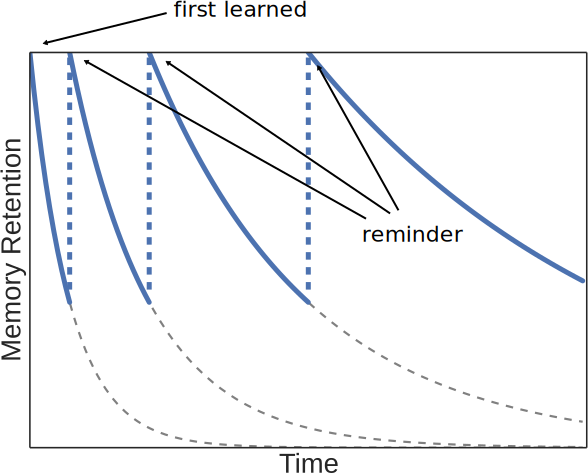
\includegraphics[width=.6\textwidth]{figure/forgetting_curves}
		\caption{Forgetting curve introduced by Ebbinghaus is given by a
			formula $R = e^{-\frac{t}{S}}$, where $R$ stands for the memory retention, $t$
			for the time and $S$ for the relative strength of memory. Ebbinghaus
			found realized that when the information is reminded again, it strengthens
			not only the memory, but also also reduces the forgetting rate.}
	\end{center}
\end{figure}

In the context of computerized adaptive practice we should look at the spacing
effect from two different points of view. In the first case we want to control
it within one session. Here we have full control over it and we work with
seconds, minutes or hours (maximally). With a fixed number of items for
practice we regulate the spacing by modifying the sequence of practiced items,
e.g. more blocking or interleaving version of
practice~\cite{ostrow2015blocking}, with variable set of items we can also
decide which items do not have to be practiced
anymore~\cite{kornell2008optimising} or which new items can be included.
Current research shows that in this specific case lies great potential, because
the sequencing has a big impact of the learning
performance~\cite{ostrow2015blocking} and people are not able \textbf{effectively} judge
which items are already learned~\cite{kornell2008optimising} and which ones
should be practiced~\cite{kornell2014focusing}.

In the second case we plan the practice over more
sessions~\cite{kang2014retrieval}. Ideally a system should decide when the
session starts and when it ends. Of course this decision is made by a user,
not by a system. We can only motivate users to practice regularly, e.g. every
day similarly how it is done by Duolingo (a system for learning
languages)~\cite{garcia2013learning}. This regularity allows us to strengthen
knowledge of already learned items and introduce new ones.

\subsection{Models Overview}

To provide appropriate content the given system must be able to model learners,
especially their knowledge. In the following section we provide brief overview
of so far available models.

\paragraph*{Rasch Model} is known as the one-parameter logistic model in item
response theory~\cite{de2008theory}. It assumes the student's knowledge about
an item is constant and can be expressed as a skill parameters $\theta$. Also
each item is assigned by a difficulty parameter $b$. Having these parameters
the probability of correct answer is given by the logistic function:

\begin{align}
P(correct|\theta,b) = \frac{1}{1 + e^{-(\theta - b)}}
\end{align}

Parameters of this model are usually estimated from data using the joint
maximum likelihood estimation~\cite{de2008theory}. In online environment it is
useful to update the parameters on the fly. For this purpose we can inspire by
Elo rating system~\cite{elo1978rating} originally devised for chess rating and
look at a student's answer on an item as a match between the student and
the item~\cite{papousek2014adaptive}. If our estimation is based only on the
first interactions between students and items, the algorithm works for constant
skills and difficulties, although the original Elo system assumes learning (changing skill).

\paragraph*{Bayesian Knowledge Tracing} is usually used model for
learning of procedural knowledge~\cite{van2013properties}. It models student's
knowledge in a hidden Markov model as a binary latent variable (either learned
or unlearned). The model has four parameters: probability the given is
initially learned, probability of learning based on one step, probability of
a wrong answer when the skill is learned (slip), and probability of a correct
answer when the skill is not learned (guess). Skill estimation is updated using
a Bayes rule using observed answer.  Several extensions of this model can be
found, e.g.  forgetting~\cite{qiu2010does}.

\paragraph*{Performance Factor Analysis} is a logistic model, but in contrast
with the Rasch model it handles learning~\cite{pavlik2009performance}. The
skill is represented as a linear combination of the item's difficulty ($\beta$)
and the number of past success ($s$) and failures ($f$) of the given student.

\begin{align}
P(correct|\beta,s, f) = \frac{1}{1 + e^{-(\beta + \gamma s + \delta f)}}
\end{align}

where $\gamma$ stands for the change of the skill associated with correct
answer and $\delta$ stands for the same in case of incorrect answer.

\paragraph*{Adaptive Character of Thought-Rational} is another logistic model
handling learning and forgetting~\cite{pavlik2005practice}. For each
presentation $i$ of the given item we track amount of time $t_i$ elapsed since
it. The activation $m$ of the given item is a function of these times:

\begin{align}
m_n(t_1, \ldots, t_n) = ln\left(\sum_{i=1}^n t_i^{-d}\right)
\end{align}

Parameter $d$ represents decay in time. To get probability a learner recalls
the given item correctly, we process the activation using logistic function,
$P(correct|m) = \frac{1}{1 + e^{m}}$.\footnote{The original model contains more
parameters and the mentioned equation is simplified. For more detail
see~\cite{pavlik2005practice}.} The model can be extended to cover also spacing
effect when we make the decay parameter dynamic, e.g. dependent directly on
spacing or the previous activation level~\cite{anderson1991reflections} (as
cited in~\cite{pavlik2005practice}).

\bigskip

\noindent
In many areas of learning of factual knowledge people enter a tutoring system
with varied prior knowledge, e.g. vocabulary or geography. The system needs to
quickly assess what a learner knows to be able to adaptively provide appropriate
content. This feature is often missing in several systems and the user is
forced to go through a lot of useless content. Our recent
work~\cite{papousek2014adaptive} similarly to~\cite{khajah2014integrating}
combines a model assuming a constant skill with another one for learning to
handle this phenomenon.  But this should go even further and models should also
provide different learning~\cite{pelanek2015modeling} and forgetting rate for
different items.  A model using a mixture of individual learning curves
implemented within Duolingo~\cite{streeter2015mixture} already covers some of
these aspects, but they do not give much attention to prior knowledge and
ignore spacing effect.  On the other side studies dealing with spacing effect
are usually based on observations in laboratory with artificial conditions, e.g.
people learn generally unknown terms to prevent prior
knowledge~\cite{kang2014retrieval} or there is no corrective-feedback given
during retrieval practice~\cite{landauer1978optimum}~(as cited
in~\cite{kang2014retrieval}) and it is questionable how all their insights will
work within an online system.

\section{Practice Control}
\label{section:practice_control}

As we already presented in the previous sections we focus on \emph{outer loop}
of user's practice~\cite{vanlehn2006behavior}, mainly within one session, that
is sequencing of items presented to the user. The considered area of learning
of facts doesn't provide sufficiently complex tasks to deal with \emph{inner
loop} (e.g. hints)~\cite{vanlehn2006behavior} and we think it is enough. The
practice itself consists of a sequence of multiple-choice and open
questions and we have to decide not only which item should be practiced, but
also whether and how many options the question should have and in case of
multiple-choice questions which items should be used as distractors. Sequencing
should also take into account spacing effect and forgetting described in
section~\ref{section:spacing_effect}.

\subsection{Sequencing}

By sequencing the items presented to a user for practice we balance between two
states: \emph{over-practice} and \emph{under-practice}. In the first case we
practice an already learned item and we waste user's time. In the second one we
stop practicing an item which is not learned yet and we will not give her a
chance learn it completely. When a system tries to avoid over-practiced
attempts, there is high chance that under-practice increases and vice versa.
How this phenomenon is important is presented in a study~\cite{cen2007over}
where its authors reported that analyzing historical data they detected more
than $50\%$ out of practice attempts as over-practiced.

In a lot of used systems a general approach for sequencing the items for
practice is based on labeling from an expert. The experts defines knowledge
components for the given domain and prerequisites among them. There are
techniques helping the ex\-perts~\cite{niznan2014using} or completely replace
them by a computer~\cite{boros2013automatic}. However, these techniques are
rarely used. Each component is a set of items and generally one item can be
included within more components. We can practice items belonging to one
component as long as the given user has mastered its prerequisites, but not the
component itself. This edge of knowledge is also known as the \emph{zone of
proximal development}~\cite{lee2005signifying}.

The mastery is detected by a model predicting user's performance and we say
that the user masters the knowledge component when the predicted probability
the user learned the component exceeds the \emph{mastery threshold} which is
usually set to~$95\%$. Mastery threshold can be viewed as parameter controlling
the relative frequency of under-practiced and over-practiced
attempts~\cite{fancsali2013optimal}. Since our model needs data about a user
to make estimation, there is some low acceptable number of attempts after the
knowledge is acquired. This \emph{lag} studied in more details
in~\cite{fancsali2013optimal}, but the study is limited for \emph{Bayesian
knowledge tracing} only. Another \emph{when-to-stop} policy is based on the
expected improvement~\cite{rollinson2015predictive}. When the system expects
the improvement below a given threshold in some knowledge component, it stops
practicing it. Low expected improvement indicates already mastered domain or
the user is unable to master it.

Similar approach is presented in~\cite{lopes2015multi}. It relies
on~\emph{multi-armed bandits}, a technique generally being able to explore
space of different parameters or strategies with respect to a given scoring
function. The authors define a structure of activities and pre-conditions
analogical to knowledge components and prerequisites and introduce two
algorithms optimizing user's learning. The first one is independent on any
model estimating user's performance, the second one uses it. Both of them take
information from experts and measure user's learning online based on progress
of the user's performance. At time $t$, the measure compares the success of the
last $\frac{d}{2}$ samples with the $\frac{d}{2}$ previous samples. Learning
can estimated by this way thanks to the fact, the system measures and improves
the user's performance at the same time. We show in
section~\ref{section:evaluation} this is not always true in some kind of
systems.

In some cases the approach using a graph of prerequisites makes sense, e.g.
in algebra we have a strong structure of prerequisites among the knowledge
components (addition and multiplication) and the choice of an item (exercise)
from the knowledge component is not so important, if we know that all
prerequisites for the given component are mastered. On the other hand in case
of a system for learning of vocabulary, individual items are independent, so we
have one item per knowledge component. Of course we can build a structure of
categories and prerequisites, but they represent a recommended study plan
rather than necessity. When a user enters the system, she can theoretically
start practicing anything.

In~\cite{papousek2014adaptive} and~\cite{papousek2015impact} we present an
approach mainly based on target difficulty. We assume we have already
estimation of user's performance for each item available in our system,
together with other descriptive information like number of interactions with
the given item, last time when the user interacted with it and so on. Since the
estimation is based only on historical data we do not need any expert's input.
On the other side we are fully dependent on the choice of target difficulty and
although there are studies about it~\cite{lomas2013optimizing,
lomas2014optimizing,jansen2013influence,papousek2015impact}, further research
has to be done in this area. Several systems has this parameter set
arbitrarily, e.g.  75\% chance of correct
answer~\cite{klinkenberg2011computer}.

As we present in section~\ref{section:spacing_effect}, learning of facts highly
relates to time and spacing effect. From this point of view the  schedule of
practice was already studied~\cite{pavlik2008schedule}, but in different
context, which is in laboratory with low number of items and without any prior
knowledge. Figure~\ref{figure:practice_progress} shows how the spacing effect
relates to the content of practice and number of practiced items.

\begin{figure}
	\begin{subfigure}[b]{.5\textwidth}
		\centering
		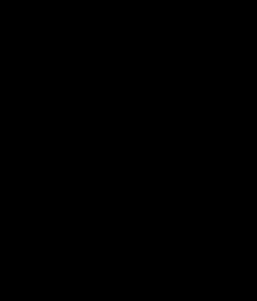
\includegraphics[width=0.9\textwidth]{figure/practice_progress_a}
		\caption{high spacing}
		\label{figure:practice_progress_a}
	\end{subfigure}
	\begin{subfigure}[b]{.5\textwidth}
		\centering
		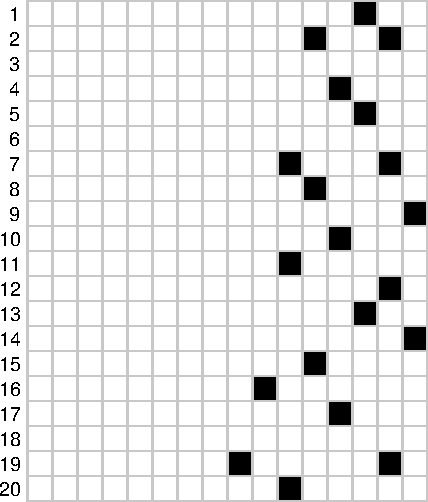
\includegraphics[width=0.9\textwidth]{figure/practice_progress_b}
		\caption{low spacing}
		\label{figure:practice_progress_b}
	\end{subfigure}
	\caption{Visualization of practice with different spacing, each column
		corresponds to an item, each row represents a discrete time unit. Black
		boxes stands for practice attempts.}
	\label{figure:practice_progress}
\end{figure}

\subsection{Questions}

Assume we have already picked an item for practice which corresponds to a
flashcard with two sides $A$ and $B$. We must specify a direction of the final
question (whether we ask for the side $A$ or $B$), e.g. in case of vocabulary
the first direction leads to an ability of understanding to foreign language
and the second one to an ability of expressing of ideas in it. In both ways we
want to achieve so-called \emph{cued recall}~\cite{carpenter2006types}.

Once we select a direction we must decide whether the question will be
open or how many options it will have. Using the options we allow a user
to guess the correct answer, so we make the question easier.
Figure~\ref{figure:options_vs_spacing} shows how the number of options relates
to difficulty of the final question together with spacing which is controlled
by sequencing. If our only goal is to make the difficulty of user's practice
appropriate, it is not clear which combination of spacing and number of options
we should use.

\begin{figure}[h]
	\begin{center}
		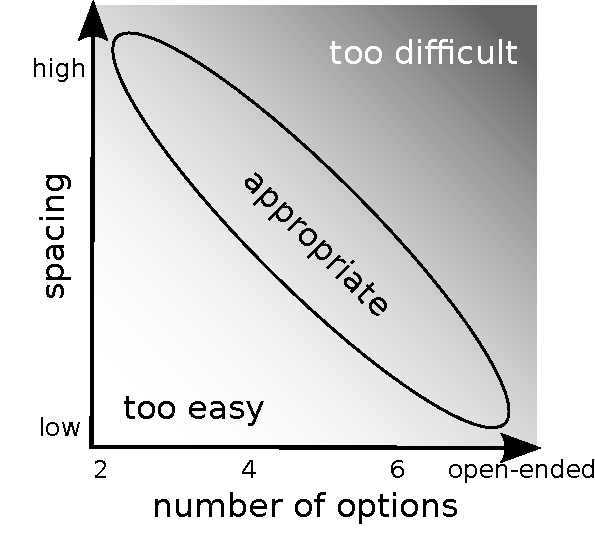
\includegraphics[width=.5\textwidth]{figure/options_vs_spacing}
	\end{center}
	\caption{Graph illustrating how difficulty depends on spacing and number of
		options. Darker background color means more difficult practice.}
	\label{figure:options_vs_spacing}
\end{figure}

The next issue is how exactly should be the options themselves be chosen. We
assume too easy options made the guess probability so high, a user wouldn't be
motivated to learn anything. The impact of competitiveness of options has been
studied in~\cite{little2015optimizing}. The study contains two experiments
where the first one does not include feedback about the correctness of user's
answer, so its results can be hardly applied within an application where the
feedback is present. And based on the second experiment where the feedback was
included, competitive options seem to be the better choice. However, the
experiment was very limited, so this phenomenon is worth further investigation.

The second aspect related to the competitiveness of the options is repeating the
same mistakes. Authors in~\cite{marsh2007memorial} describe experiments where
wrong answer in the final test are correlated to wrong answers within a
preparation phase where multiple-choice question were used. These observation
should be definitely taken into account when the options are built within an
adaptive system for practice.

\section{Evaluation}
\label{section:evaluation}

Any effort to improve any kind of intelligent tutoring system would be useless
if we were not able to measure some of its features. Design of these
adaptive systems and choice of their parameters are really difficult and then
their adaptive behavior is hard to predict, so it is crucial to be sure they
meet our expectations. Generally we want to improve user's learning, but due to
the fact the systems are often used during user's free time, we must also
ensure user's willingness to use the system. How these things can relate to each
other is studied in~\cite{lomas2013optimizing}.

Since a lot of systems collect data about user's performance and their
behavior is based on models predicting the performance, its natural to
evaluate new models using the historical data with respect to accuracy. We can
also try to find whether the behavior of the system would change, if it used a
different model. The second possibility is to deploy a new feature, collect new
data and then see what has changed. This way is really expensive, because we
spend user's time for testing of our system instead of learning something. We
also risk negative impact on users. The last way how to examine our ideas is to
use synthetic data. Generating synthetic data is cheap, there is no risk, but
we must work with a lot of assumptions which can limit us.

\subsection{Historical Data}

Typical data about user's performance contains a list of solved tasks and
binary information whether the user's solution was correct ($1$) or incorrect
($0$). A model predicting user's performance returns values from the interval
$[0, 1]$. Based on this we can fit a new model on a subset of data a test its
predictions compared to the rest of data. From the viewpoint of accuracy there
is a set of more or less appropriate metrics depending on the fact whether an
absolute or relative value of the prediction is important, which is more deeply
described in~\cite{pelanek2014brief}.  From a practical point of view the
accuracy is not the only important aspect of the predictive
model~\cite{huang2015framework}. It also gives us deeper insight into a domain.
Regarding this it is useful the given model holds some of the key assumptions,
e.g. a user's knowledge increases with each exercise or while fitting its
parameters converges to similar values regardless division of the data.

Similar area to adaptive systems for practice are recommender systems, e.g. for
books or movies. These systems also work with predictive models to serve
appropriate content to their users. There are
studies~\cite{cremonesi2010performance} how the accuracy of a model relates to
behavior of a recommender system as a whole using only historical data. It
would be nice to have the same for educational systems. Something similar is
presented in~\cite{yudelson2015small} where the authors quantify saved user's
time to get mastery in case of a better model. However, it is questionable how
valuable these observations are. In an extreme case, a model predicting $100\%$
performance would be the best from this point of view, but it is not definitely
helpful.

\subsection{New Data}

Classical approach to examine the impact of the given system on the user's
behavior is to follow the \emph{pre-test} $\rightarrow$ \emph{intervention}
$\rightarrow$ \emph{post-test} experimental design~\cite{dimitrov2003pretest}.
Usually the researchers has a full control over the participants, often in
laboratory, but also in online environment where the participants are motivated
to finish the whole experiment by money, e.g. in~\cite{maass2015how}. In test
phases they are assessed with respect to a measured property and the
intervention phase they use the system for the given amount of time. Although
this approach is very helpful and brings a lot of interesting observations, it
does not scale.

In online environment we need to periodically deploy new features and
test them only on a subset of users, before we publish them
completely~\footnote{This process is also known as \emph{canary deployment}.}
.Doing this kind of online A/B testing opens new possibilities to
us~\cite{stamper2012rise}, we can collect large volume of data and make a
cycle of hypothesis testing faster. Unfortunately users in online environment
enter and quit a system anytime, so we can hardly adopt a method of
pre/post-testing. From this reason many studies are focused only on measuring
time a user spent in a system or number of
interactions~\cite{papousek2015impact,monterrat2015player}
rather than improvement in her performance.

\begin{figure}[h]
	\begin{center}
		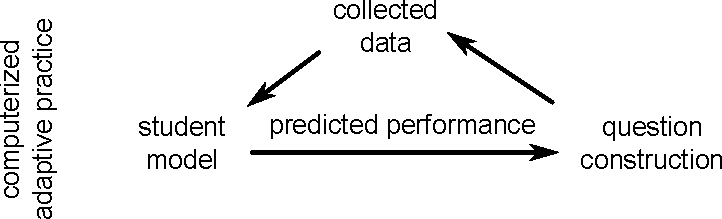
\includegraphics[width=.7\textwidth]{figure/interaction_loop}
	\end{center}
	\caption{Schema illustrating the interaction loop between student model and
		question construction~\cite{niznan2015exploring}.}
	\label{figure:interaction_loop}
\end{figure}

On the other side authors in~\cite{lomas2013optimizing} analyze both the time
and the performance via fitting learning curves on collected data, but it is
not clear whether the data are not influenced by the collection (higher error
tolerance can naturally lead to higher error rate and it does not say anything
about learning).  Our system for practicing of geography is aimed at a
predefined success rate~\cite{papousek2014adaptive}, so we can not simply use
the collected data to measure the user's performance. Although the interaction loop
shown on Figure~\ref{figure:interaction_loop} is present in many systems, it is
usually ignored.

Another interesting issue is how exactly we should perform the online
experiments to maximize the amount of retrieved information and minimize
experimental time~\cite{liu2014towards}. Here is great potential in techniques
like multi-armed bandits~\cite{liu2014trading} which can be used to
automatically optimize values for parameters of the practice over populations
of users.

\subsection{Synthetic Data}

Using simulated learners we easily generate synthetic data. The assumptions for
simulation are usually derived from real traffic. We know the ground truth, how
difficult items are, when a learner mastered a knowledge component and so on.
This allows us to investigate issues which could not be otherwise, like
detection of mastery~\cite{fancsali2013optimal}, learning
curves~\cite{fancsali2013simulated} or the interaction between a model
predicting user's performance and a system as a
whole~\cite{niznan2015exploring}. In~\cite{niznan2015exploring} we assume that
the optimal practice is given by a set of practiced items using a model with an
access to the ground truth and we compare practiced items with other models to
this one. Authors in~\cite{lopes2015multi} also use simulated learners before
the experiments with real people and state the practice should be personalized
which leads to varied practice sequences. More diversity is in data, better
system is.

Experiments with synthetic data are limited by the assumptions we have for the
simulated learners. On the other hand, fewer assumptions we want to bring lead
to simpler experiments, e.g. in our study we did not want to assume anything
about learning, so our simulated practice does not contain repeated
interactions with the same item.

\chapter{Aims of the Thesis}
\label{chapter:aims_of_the_thesis}

\section{Objectives}

The main aim of the thesis is to make learning of factual knowledge more
efficient. We believe we can design strategies for practice of
multiple choice questions in online environment focused on the proper
sequencing of questions and adjustment their difficulty to learner's needs,
both leading to better learning efficiency. Although the strategies will be
applied and evaluated mainly within an application for practice of geography,
the found results should be easily applicable to other similar domains like
learning of vocabulary.

The particular goals are as follows:

\vspace{-.3cm}
\paragraph*{Model:} As we describe in section~\ref{section:models} the crucial
part of computerized adaptive practice is a model describing learner's
knowledge. We will investigate models predicting learner's performance during
learning taking into account spacing effect and forgetting. These factors are
really important in case of factual knowledge. The considered model should
cooperate witch existing model for prior knowledge~\cite{papousek2014adaptive}
and should be applicable not only offline, byt also in online environment. It
will be deployed within a real system for adaptive practice.

\vspace{-.3cm}
\paragraph{Practice Control:} We plan to develop strategies for sequencing and
question construction with focus on appropriate difficulty, spacing effect and
suitable distractors for multiple-choice questions. We want to introduce a
mechanism of variable difficulty of distractors, e.g. in the beginning of the
practice the distractors will be easy, later they will be more difficult. The
strategies will highly rely on the predictive model, but we will also build on
existing research using in-lab experiments.

\vspace{-.3cm}
\paragraph{Evaluation:} In section~\ref{section:evaluation} we address an issue
of evaluation in case of intelligent tutoring systems. From this reason a big
part of the thesis will be dedicated to the methodology of evaluation:
\begin{enumerate}
	\item We will propose a methodology to evaluate the impact of adaptive
		practice on user's learning in online environment. We want to cover both
		learning efficiency and learner's willingness to use the tutoring system.
		We will apply the designed methodology to evaulate real system for adaptive
		practice.
	\item Using synthetic data we will investigate further the interaction loop
		between the student's model and the algorithm for question construction,
		mainly a role of the mechanism of difficulty adjustment based on a learner's
		history.
\end{enumerate}

\section{Expected Outputs}
\begin{enumerate}
	\item The text of the thesis presenting both theoretical and experimental
		results.
	\item Publicaly available system for computerized adaptive practice
		implementing developed algorithms for practice control and student's
		model.
	\item Reviewed publications on relevant international conferences and in
		journals.
\end{enumerate}

\noindent
I am currently working on a journal publication:

\begin{itemize}
	\item \textbf{Learner Modeling and Adaptive Practice of Facts:}\\
		I am extending an already published analysis~\cite{papousek2015impact}
		examining the impact of adaptive practice on user's behavior, mainly
		focused on target difficulty. The paper will be published in \emph{User
		Modeling and User-Adapted Interaction}.
\end{itemize}

One journal paper is already in review process of \emph{Journal of Learning
Analytics}:

\begin{itemize}
	\item \textbf{Adaptive Geography Practice Data Set:}\\
		We published the data set collected by \url{www.slepemapy.cz}. The paper
		describes the data set.
\end{itemize}

In the future I plan to write publications about the impact of computerized
adaptive practice on learning with contrast to its impact on willingness of
users to stay in the tutoring system and self-reported perception.

\section{Proposed Plan of Work}

\begin{tabularx}{\textwidth}{rX}
	\rowcolor{white}
	\textbf{Autumn 2015} &
		\begin{enumerate*}
			\item Design and implementation of methodology for evaluation of the impact
				of adaptive practice on user's learning.
			\item Evaluation of already existing algorithm for practice control using the
				developed methodology.
			\item Deployment of a new version of \url{www.slepemapy.cz}
				being able to adopt a new student model.
		\end{enumerate*}\\
	\rowcolor{white}
	\textbf{Spring 2016} &
		\begin{enumerate*}
			\item Design and implementation of a new student's model of learning of
				factual knowledge.
			\item Development of strategies for practice control cooperating with a
				proposed student's model.
		\end{enumerate*}\\
	\rowcolor{white}
	\textbf{Autumn 2016} &
		\begin{enumerate*}
			\item Evaluation of proposed strategies.
			\item Experiments with synthetic data.
		\end{enumerate*}\\
	\rowcolor{white}
	\textbf{Spring 2017} &
		\begin{enumerate*}
			\item Finishing and submitting the thesis.
		\end{enumerate*}
\end{tabularx}

\chapter{Achieved Results}
\label{chapter:achieved_results}

\section{System for Adaptive Practice of Geography}

We have implemented an adaptive system providing adaptive practice of geography
facts available at~\url{www.slepemapy.cz}~\cite{papousek2014adaptive}. It
estimates user's and based on the estimation it asks questions of suitable
difficulty. These questions are open or multiple-choice with from 2 to 6
options, they are of 2 different directions ("Where is Germany?" or "What is
the name of the highlighted country"), see
figure~\ref{figure:example_question}. The questions are then answered using
"outline map". After a sequence of 10 answers the system shows to user a
feedback on her success.  Users can also access a visualization of their
knowledge using an open learner model.

\begin{figure}[h]
	\begin{center}
		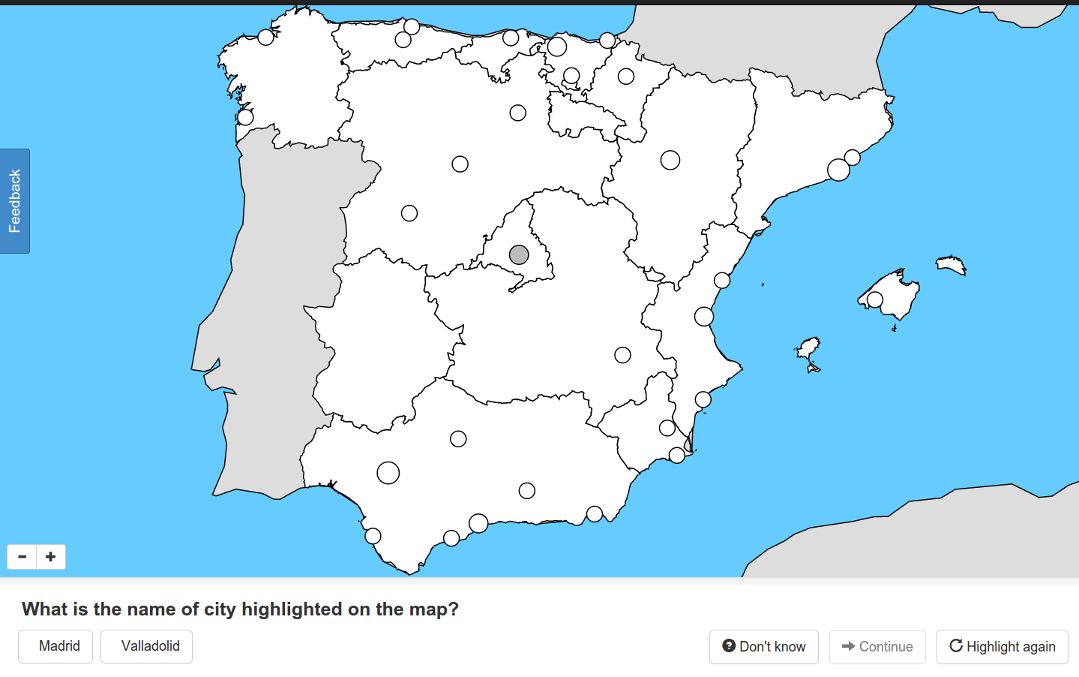
\includegraphics[width=\textwidth]{figure/slepemapy_spain_highlighted}
		\caption{An example of a question asked by \url{www.slepemapy.cz}.}
		\label{figure:example_question}
	\end{center}
\end{figure}

The design of our system is decomposed into 3 steps and each step is handled
independently. More detailed description is available
in~\cite{papousek2014adaptive, papousek2015impact}.

\begin{enumerate}
	\item \emph{Estimation of prior knowledge}. The system tries to estimate the
		probability a user $u$ knows an item $i$ before the first question
		about this item. The estimate is based on previous answers of the user $u$
		and on answers of other users about the item $i$.
	\item \emph{Estimation of current knowledge}. In this case the system
		estimates the probability a user $u$ knows an item $i$ based on the
		estimation of prior knowledge and a sequence of previous answers of the
		user $u$ about the item $i$.
	\item \emph{Question construction}. Based on the estimation of user's
		knowledge and other additional information the system constructs suitable
		question for the given user.
\end{enumerate}

\begin{figure}[h]
	\begin{center}
		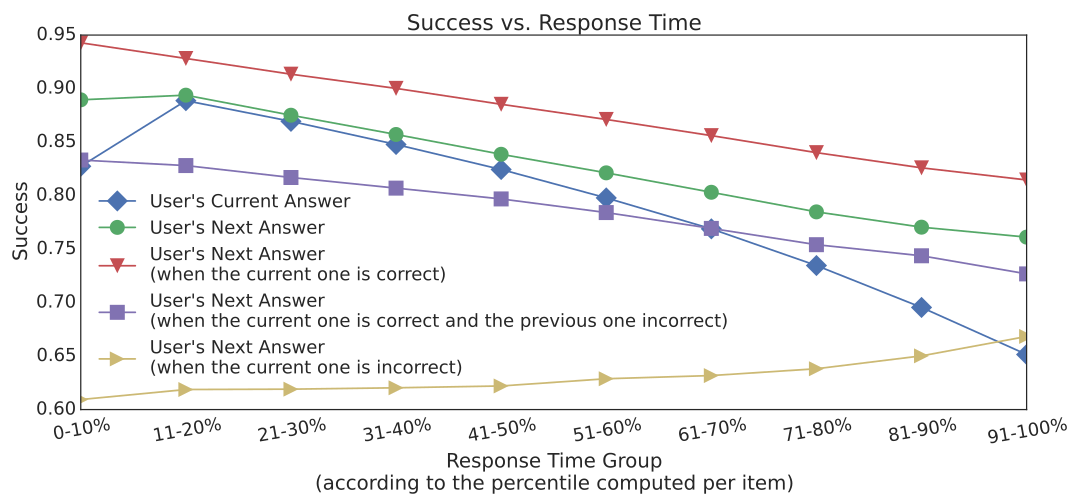
\includegraphics[width=\textwidth]{figure/response_time}
		\caption{Response times and probability that the (next) answer is correct~\cite{papousek2015analysis}.}
		\label{figure:response_time}
	\end{center}
\end{figure}

The system is available for free without any need of registration. However, we
offer possibility of signing up to help our system with tracking user's
history. However, we do not collect any information about the identity of users
(e.g. sex or age). So far we collected more than \numprint{11000000} answers
from more than \numprint{100000} (mostly Czech) users. Monthly we collect $\pm$
\numprint{1000000} answers from \numprint{10000} users. The traffic is lower at
weekends and during holidays, which indicates the system is used by students
from schools. This hypothesis is also supported by the traffic analysis during
one day~\cite{stanislav2015factual}. There are peaks in traffic corresponding
to lessons at schools in Czech Republic.

The collected data set serves as an interesting input for further research
within Adaptive Learning Group\footnote{\url{www.fi.muni.cz/adaptivelearning}},
e.g.~\cite{pelanek2015modeling} modeling students' memory or
\cite{niznan2015student} modeling prior knowledge.
Figure~\ref{figure:response_time} shows the relationship of response time and
correctness of an answer, e.g. in case of the wrong answer longer response time
leads to higher probability the next answer will be correct. On the other side
in case of correct answers, it is exactly the opposite. This observation could be
used to improve a model for current knowledge.

\section{Impact of Adaptivity}

In~\cite{papousek2015impact} we analyze the impact of adaptivity of our system
on user's behavior. We mainly focus on the time spent in the system expressed
by the number of answers per user. We performed online AB experiment to examine
the role of the designed algorithm for question construction and its
parameters. As we describe in section~\ref{section:practice_control} for the
question construction we firstly need to select an appropriate item and secondly
we choose number of options and options themselves.

In the first experiment we compare our approach to algorithms where at least
one of these two steps is random. We found out that both parts of the algorithm
are important. Using random version of the first or the second part leads to
the similar results as in case of the completely random algorithm.

Since the selection of an appropriate item for practice is based on the target
difficulty, we performed the second experiment to find the optimal value for
this parameter. Unfortunately we were not able to find any significant
difference for different values of target difficulty with respect to the number
of answers per user. This is probably caused by the fact that users can choose
different practice contexts (maps) and for different contexts our system
behaves differently, e.g in case of European countries the system can not
provide sufficiently difficult practice for some users and on the other side
for African countries there is sometimes a problem to pick sufficiently easy
questions. Based on this we look not on the target difficulty with respect to
the number of answers, but on the real difficulty with respect to self-reported
perception\footnote{We ask users to evaluate the practice after $30$, $70$,
$120$ and $200$ answers, whether it is "Too difficult", "Appropriate" or "Too
easy".}. Using heuristics based on IP address we also detect in-school users
and compare them to out-of-school users. For analysis we divide users according
to their success to buckets and for each bucket we compute the percentage of
"Too difficult", "Appropriate" and "Too easy" records, see
figure~\ref{figure:feedback_by_success}.

\begin{figure}[h]
	\begin{center}
		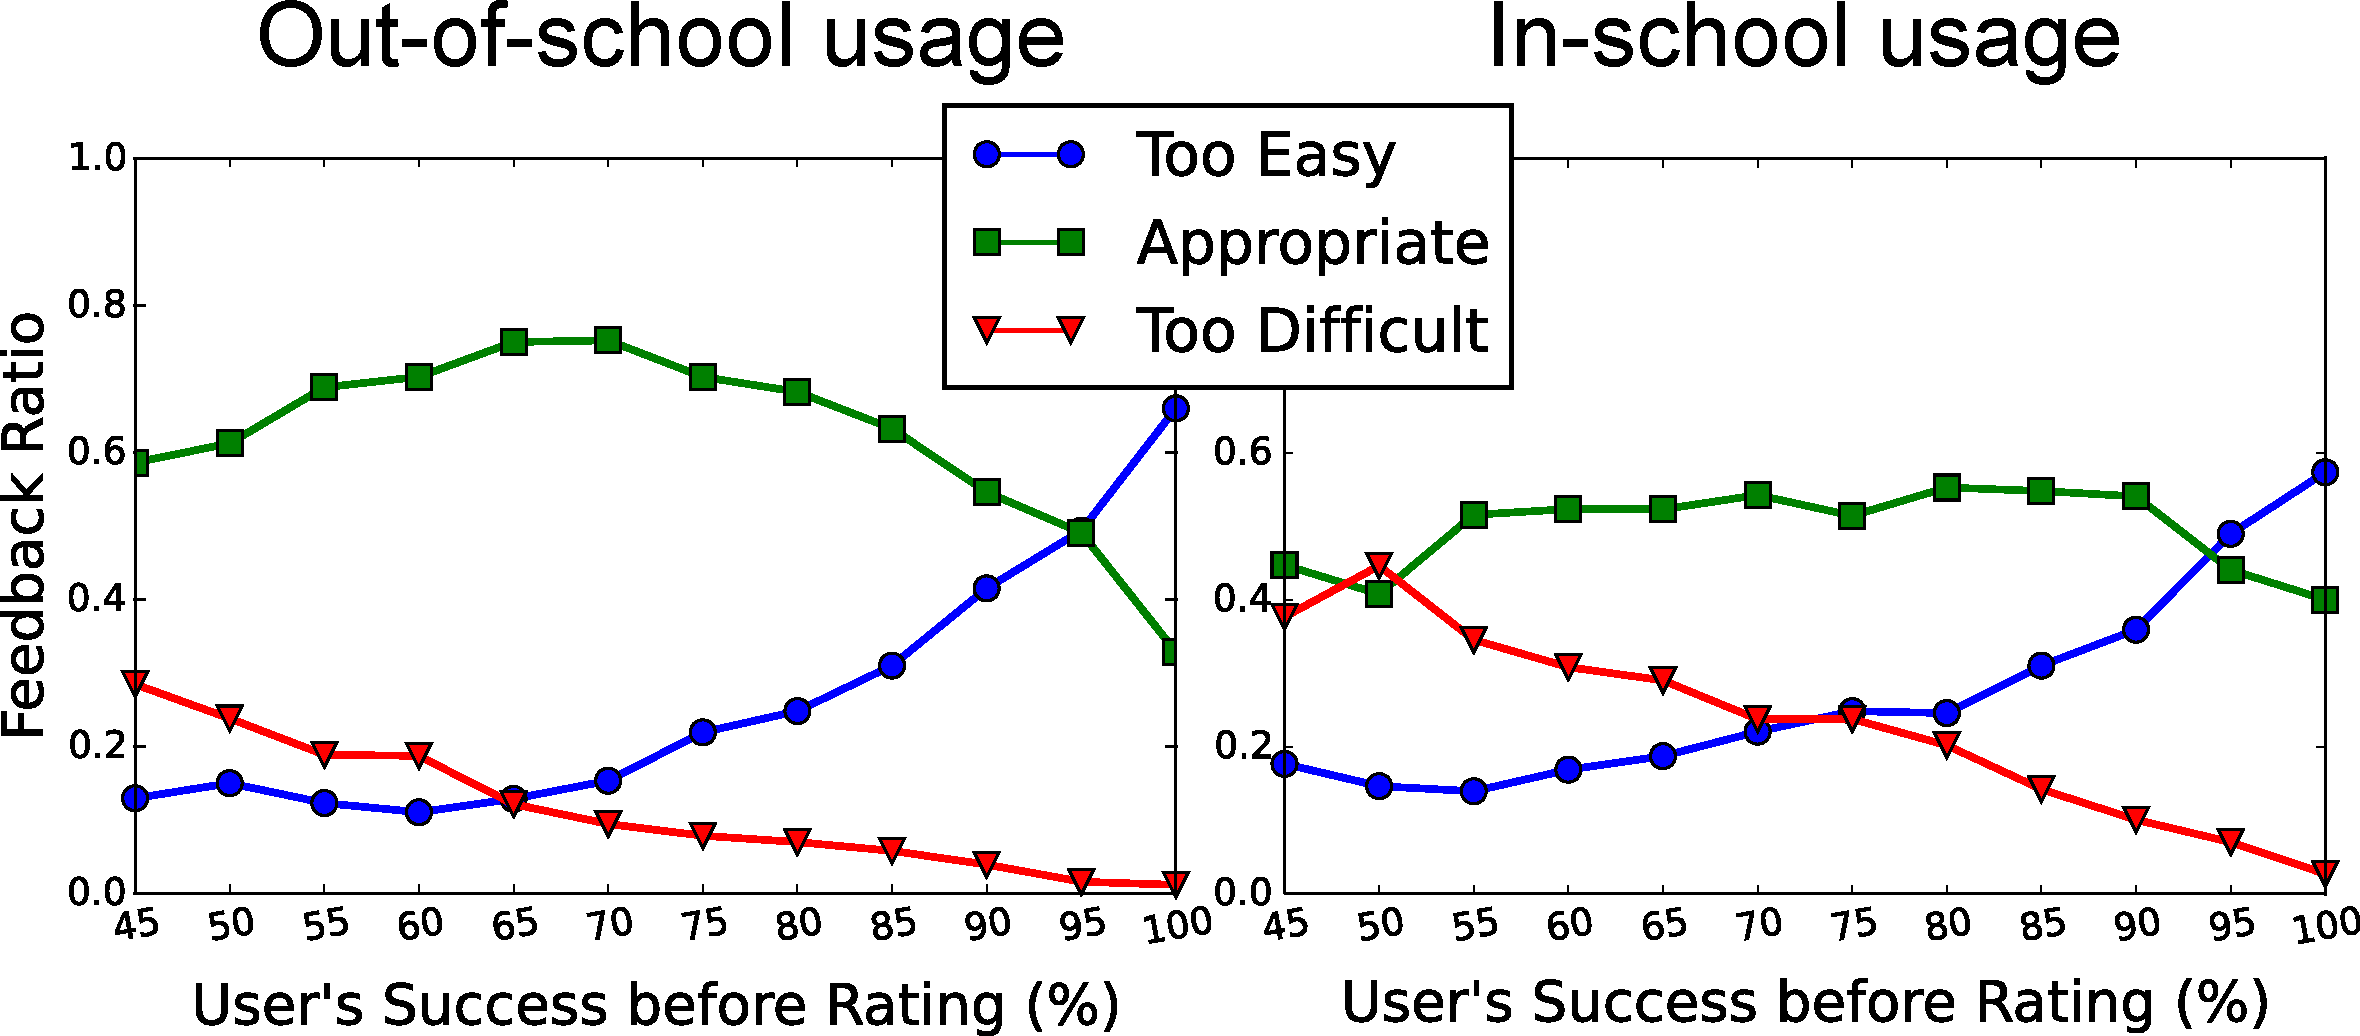
\includegraphics[width=\textwidth]{figure/feedback_by_success_overview}
		\caption{Explicit feedback given by students according to their previous
			real success rate. ~\cite{papousek2015impact}.}
		\label{figure:feedback_by_success}
	\end{center}
\end{figure}

The target difficulty is not constant in our system, we adjust it based on the
user's history. For successful users we make the practice more difficult, for
less successful the practice will be easier. This adjustment would make the
choice of the target difficulty less important, so we were interested whether
it has a positive impact on users. The last experiment shows that the group
having the adjustment enabled answers more questions than the group without it.

\section{Interaction Loop}

Since we adaptively collect the data, we analyze it and then we try to improve
the system using the acquired insights, we have to take into account the
interaction shown on figure~\ref{figure:interaction_loop}.
In~\cite{niznan2015exploring} we investigate this interaction loop and a role of
small differences in predictive accuracy using synthetic data. We generate data
using the ground truth model simulating usage of simplified question
construction algorithm. There are 200 items and 5000 students available in the
system and each student practices 50 items. Each item is practiced by the given
student at most once.

\begin{figure}[h]
	\begin{center}
		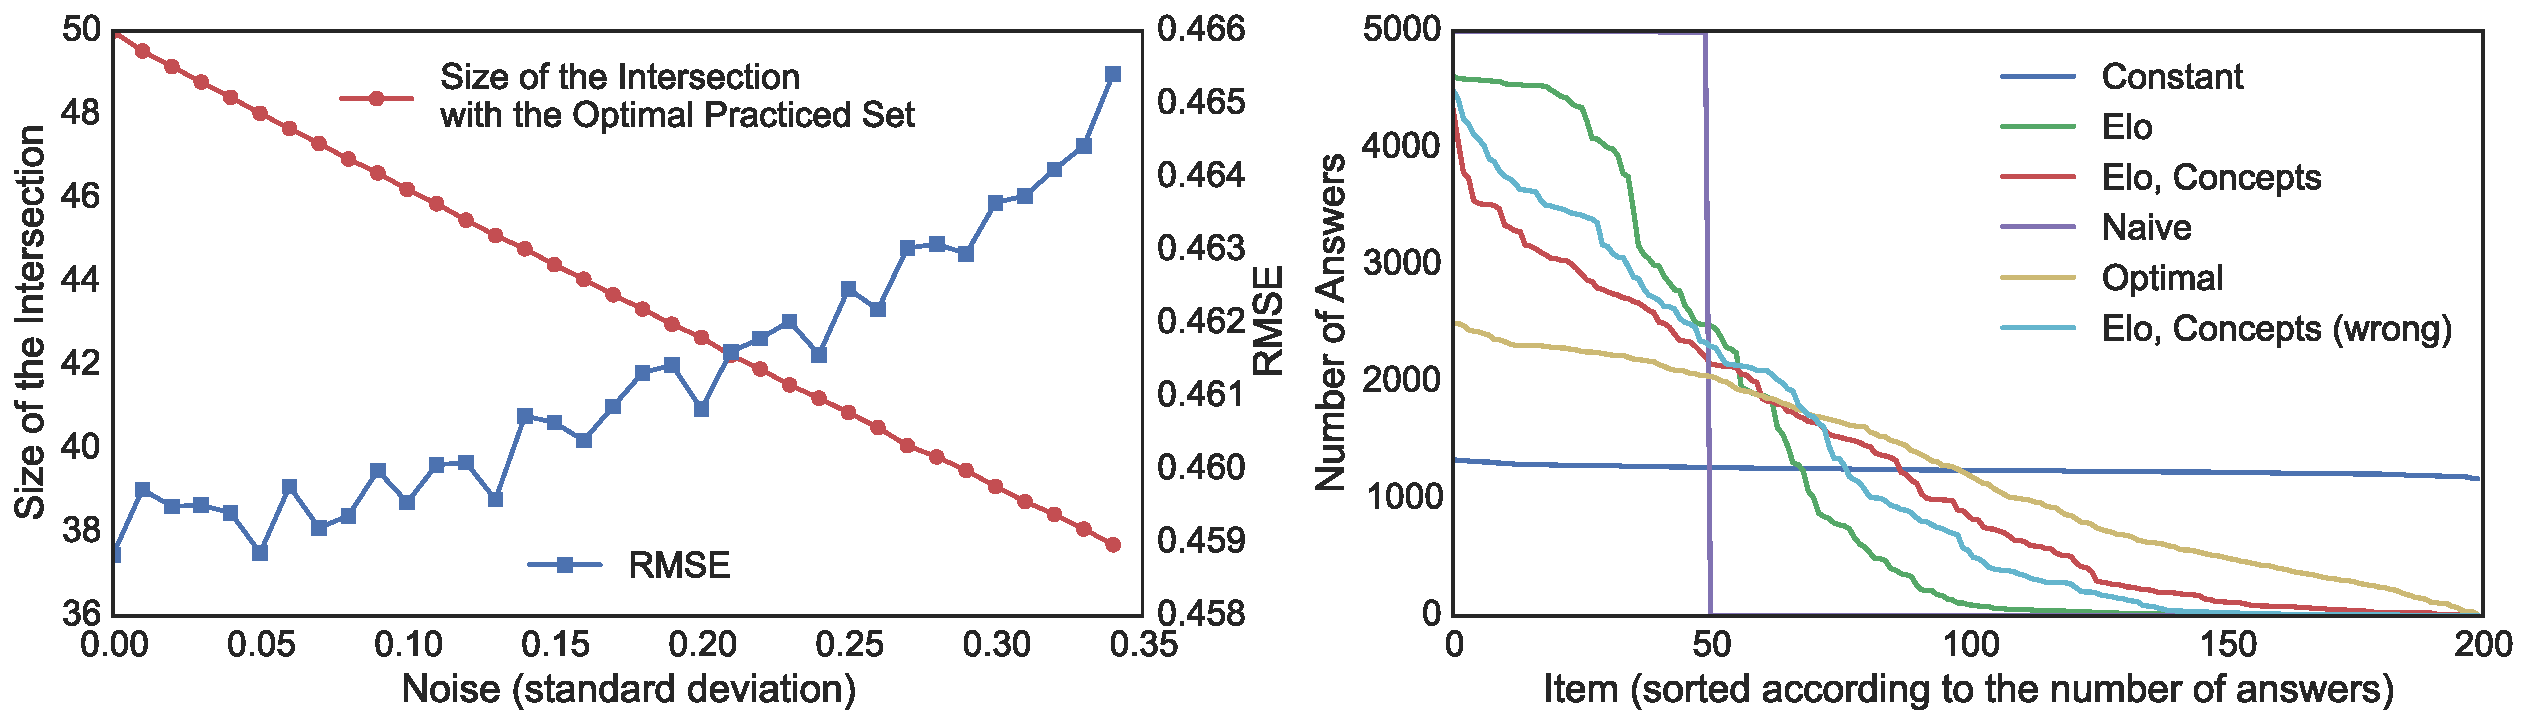
\includegraphics[width=\textwidth]{figure/noise_vs_intersection_number_of_answers}
		\caption{Size of the intersection with the optimal practiced set of items and RMSE
			depending on Gaussian noise in optimal model (left side). Distribution of answers over
			the items based on the given model (right side)~\cite{niznan2015exploring}.}
		\label{figure:feedback_by_success}
	\end{center}
\end{figure}

Using the ground truth model we declare the practiced set
optimal, then we use a different model and see how a new practiced set
differ from the optimal one. In one experiment we gradually add more and more
noise to the ground truth model and look at the practiced set of items. We
found out that a relatively small noise leading to a small \emph{root mean
square error} (RMSE) has a big impact on the practice, see left side of
figure~\ref{figure:feedback_by_success}. In other experiment we look at the
distribution of collected data across the items. Using the ground truth model
we collect more uniform data than for the other models (except one
corresponding to completely random uniform distribution), see right side of
figure~\ref{figure:feedback_by_success}. This shows a risk we face when our
system uses a bad model. We did even more analysis related to the interaction
loop, for more details see~\cite{niznan2015exploring}.

\chapter{Author's Publications}

\begin{enumerate}
	\item \bibentry{papousek2015impact}

		\textit{I performed online experiments examining the algorithm for practice
			control with respect to the user's motivation and then analyzed the collected
			data.}
	\item \bibentry{niznan2015exploring}

		\textit{I did an analysis of feedback loop between a model describing
			user's knowledge and an algorithm for practice control collecting the
			data. I also examined the impact of the model and its precision on data
			collection.}
	\item \bibentry{papousek2015analysis}

		\textit{I analyzed the relation of response time spent  and correctness of answers.}

	\item \bibentry{papousek2014adaptive}

		\textit{I implemented the predictive model and the algorithm for practice
			control within an application providing practice of geography. I designed
			the mechanism of difficulty adjustment and selection of distractors in case of
			multiple-choice questions.}
\end{enumerate}

\bibliographystyle{plain}
\bibliography{proposal}

\appendix
\chapter{Enclosed Publications}
\section{Impact of Adaptive Educational System Behaviour on Student Motivation}
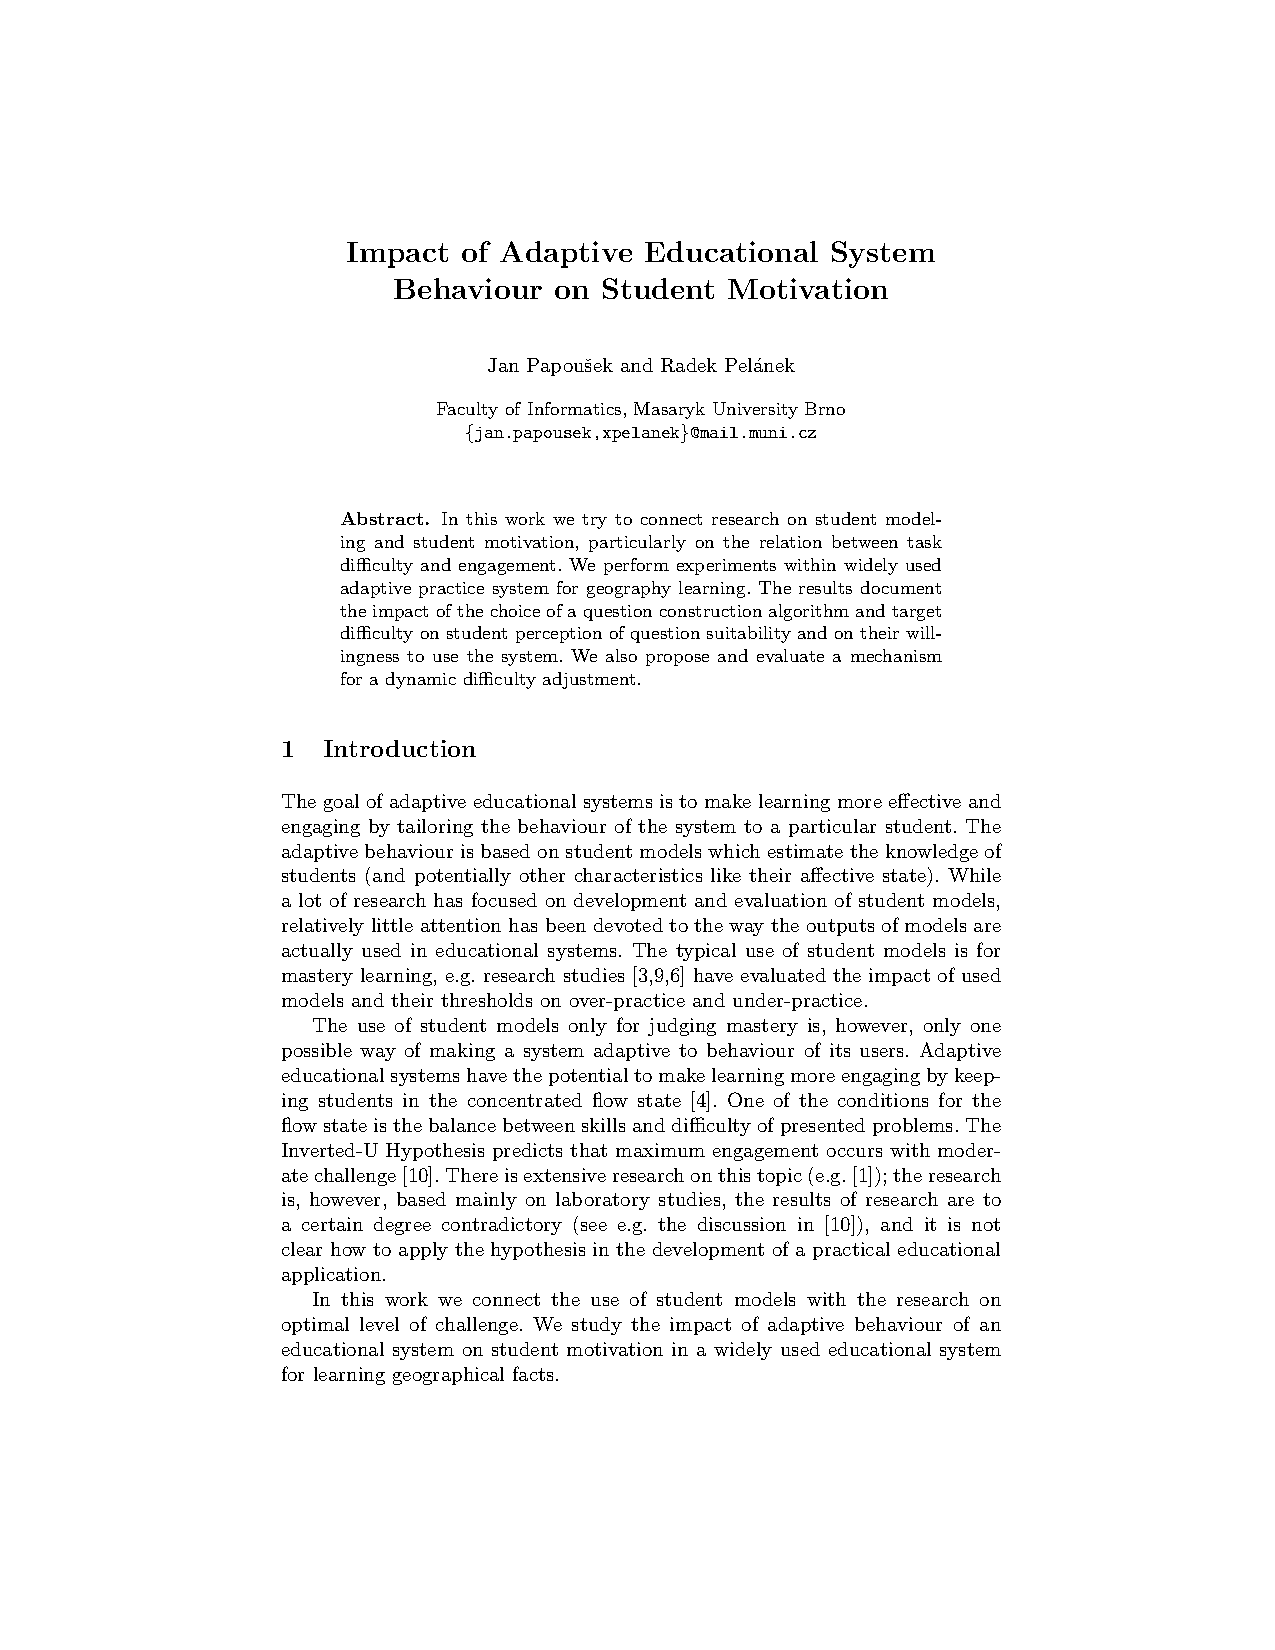
\includepdf[pages=-]{paper/papousek2015impact.pdf}
\section{Exploring the Role of Small Differences in Predictive Accuracy using  Simulated Data}
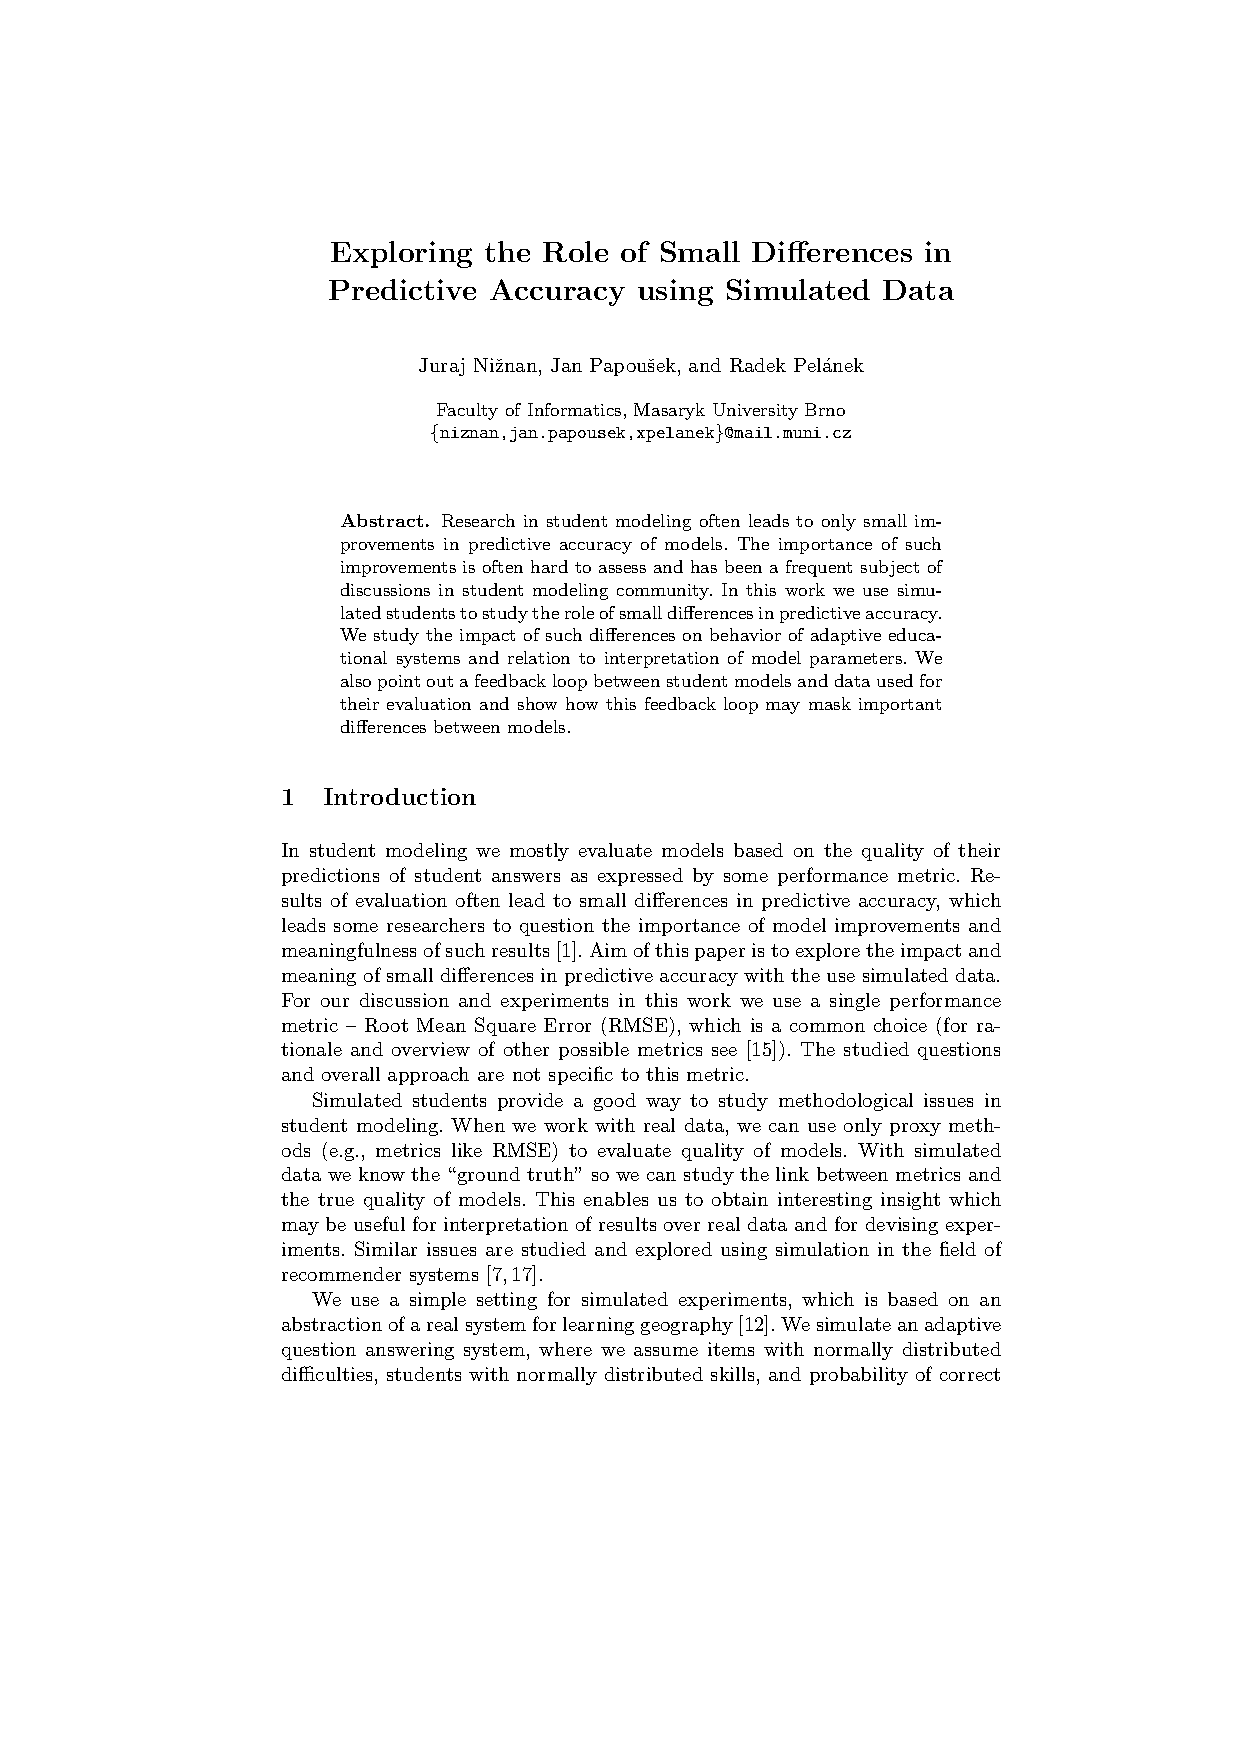
\includepdf[pages=-]{paper/niznan2015exploring.pdf}
\section{An Analysis of Response Times in Adaptive Practice of Geography Facts}
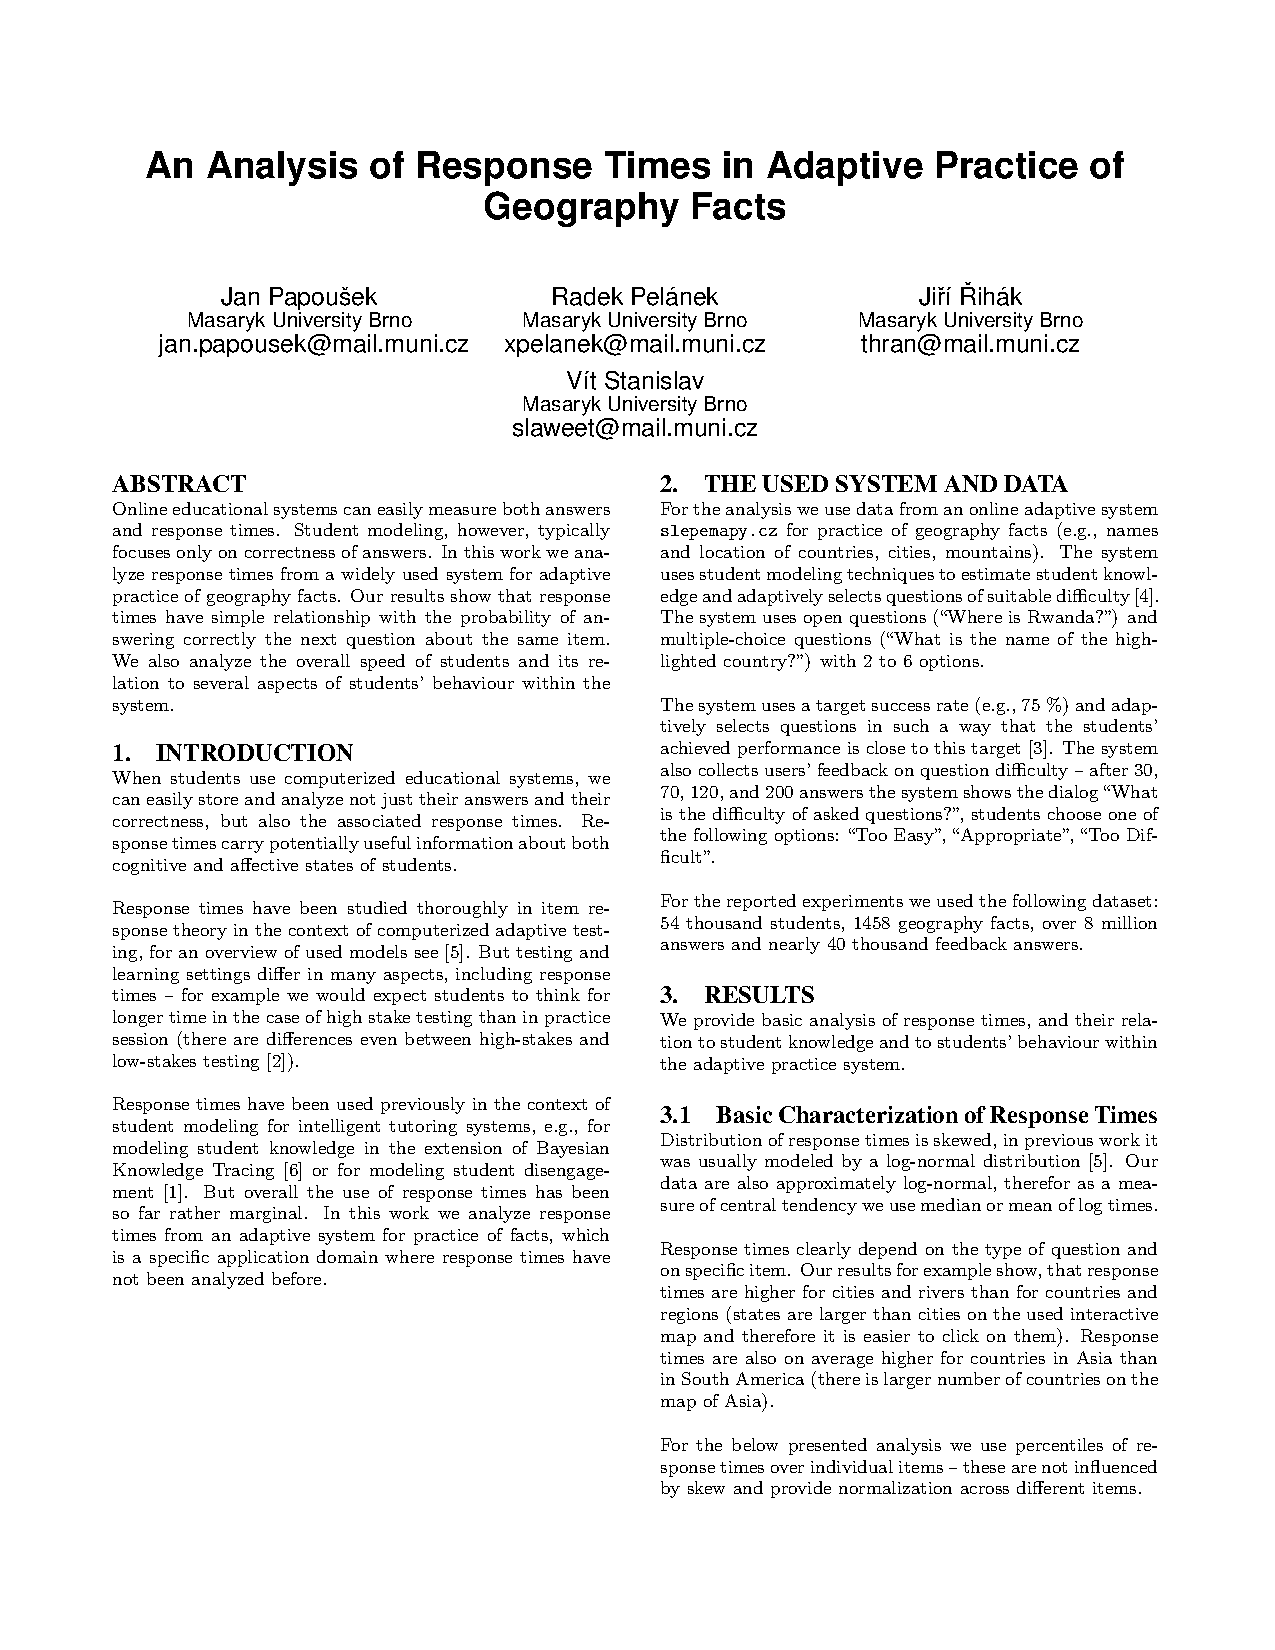
\includepdf[pages=-]{paper/papousek2015analysis.pdf}
\section{Adaptive Practice of Facts in Domains with Varied Prior Knowledge}
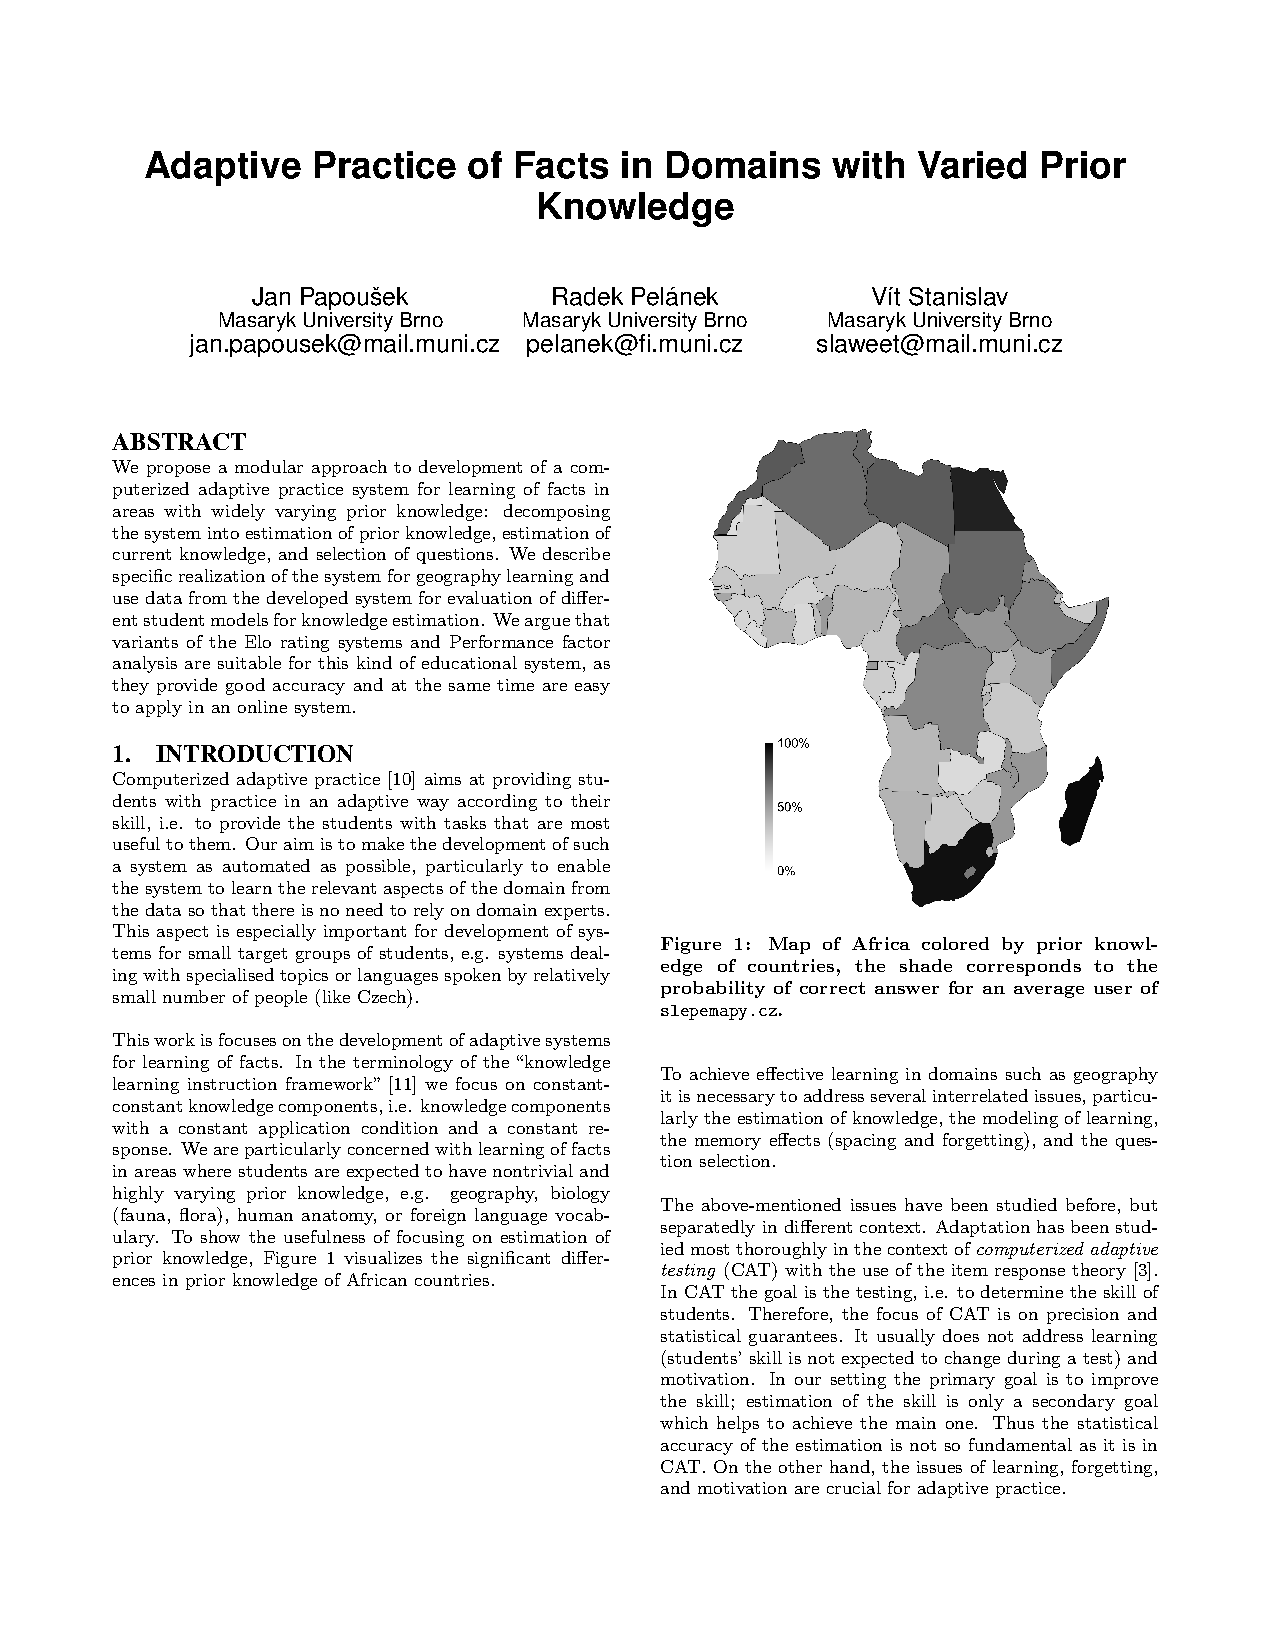
\includepdf[pages=-]{paper/papousek2014adaptive.pdf}

\end{document}
